\documentclass[11pt]{jarticle}
\usepackage{graphicx}
\usepackage{wrapfig}
\usepackage{ascmac}
\usepackage{geometry}
\usepackage{url}
\usepackage{fancyhdr}
\geometry{body={178mm,242mm},columnsep=8mm}
\usepackage{makeidx} %索引
\makeindex

\makeatletter
\newcounter{qnum}[section]
\setcounter{qnum}{0}
\def\theqnum{問\thesection.\the\c@qnum}
\def\question{\refstepcounter{qnum}%
  \vspace{3mm}\noindent\textbf{[\theqnum]}~}

%%% index

\def\bfindex{\@ifnextchar[{\@bfindex}{\@@bfindex}}
\def\@bfindex[#1]#2{\textbf{#2}\index{#1@#2}}
\def\@@bfindex#1{\textbf{#1}\index{#1}}

\def\nmindex{\@ifnextchar[{\@nmindex}{\@@nmindex}}
\def\@nmindex[#1]#2{#2\index{#1@#2}}
\def\@@nmindex#1{#1\index{#1}}
\makeatother

%\def\question{\noindent\textbf {[問題]}}
%\newenvironment{vscreen}{\begin{screen}\begin{verbatim}}{\end{verbatim}\end{screen}}


\begin{document}
\pagestyle{empty}
% \rule{\linewidth}{0.5pt}
\begin{center}
{\LARGE LEGO MindStormのNXCによる制御プログラミング}
\end{center}
\begin{flushright}
\today 版\\
西井 淳
\end{flushright}
\vspace{-0.6cm}
\rule{\linewidth}{0.5pt}

\vspace{-0.6cm}
{\small
%\begin{screen}
  \tableofcontents
%\end{screen}
}

%\newpage
\pagestyle{fancy}
\def\baselinestretch{1.05}


\section{はじめに}

\begin{wrapfigure}[13]{r}{7cm}\vspace{-1cm}
\begin{center}
  \resizebox{5cm}{!}{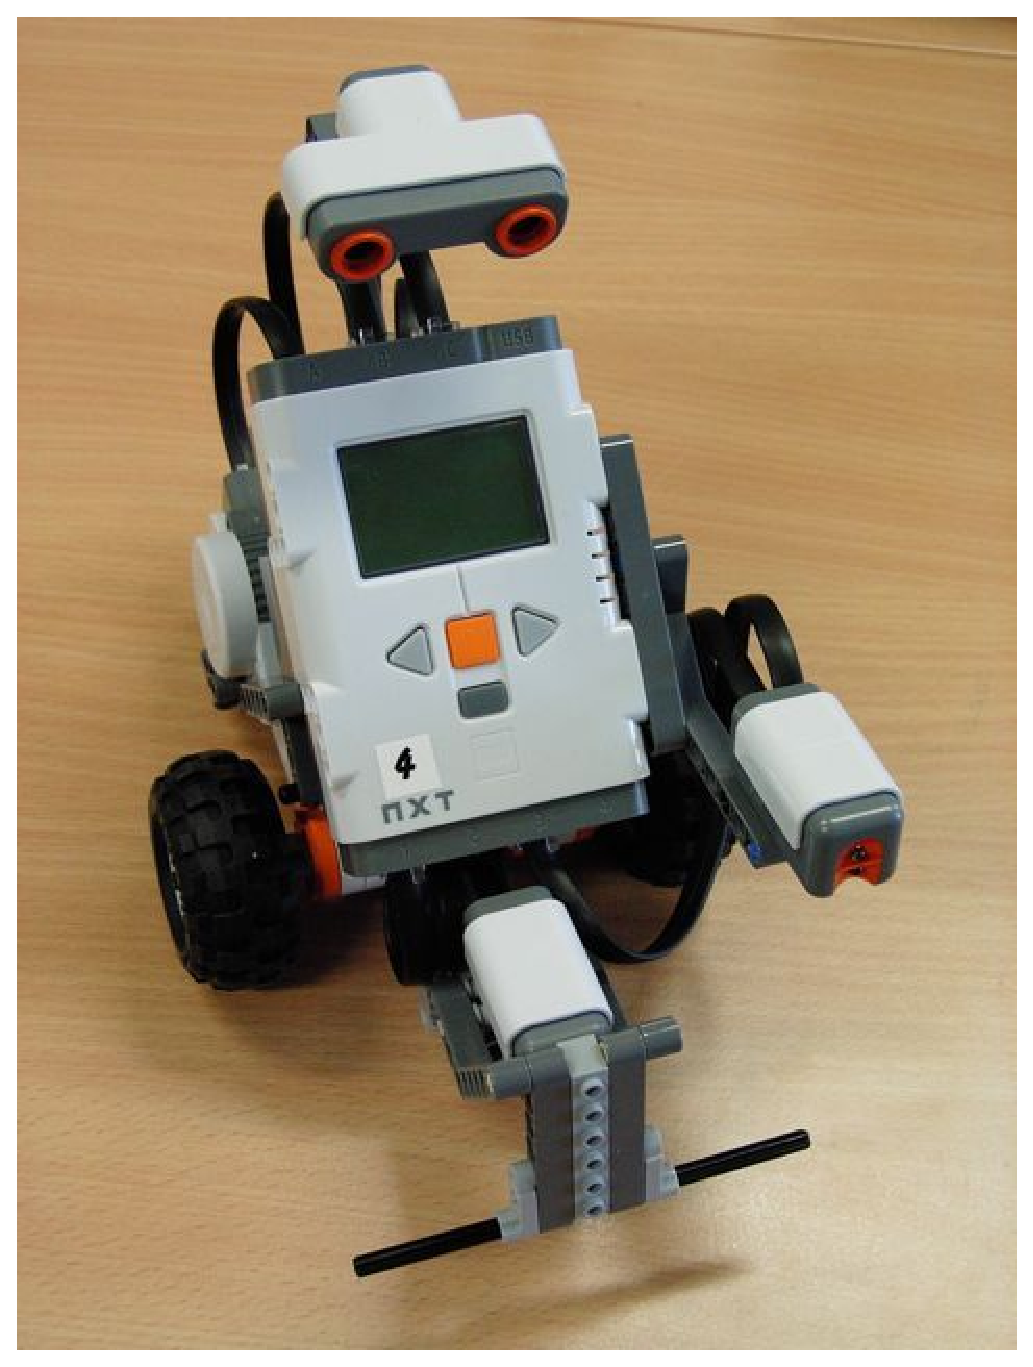
\includegraphics{images/mindstorm.eps}}
\end{center}
\end{wrapfigure}

\nmindex{LEGO MindStorm}\index{MindStorm}はLEGOがMITと共同開発したロボッ
ト制御の学習用キットです。
本テキストでは,LEGO MindStormをプログラミング言語\nmindex{NXC}(Not
eXactly C)を使って制御する方法を説明します。
NXCはC言語と似ていますが,簡単にMindStormを制御できるようにC言語と異なる点
もいろいろあります。
また,NXCプログラミングのための統合開発環境\nmindex{Bricx}も開発されています。

なお、本テキストはDaniele Benedettelli著の``Programming LEGO NXT
Robots using NXC'', John Hansen著の''Not eXactly C (NXC) Programmer's
manual''をもとにして短くまとめたものです。
いずれも\url{http://bricxcc.sourceforge.net/nbc/nxcdoc/}からダウンロー
ドできますし,Bricxにも添付されているので、詳細を知りたい人は見てくだ
さい。


\section{準備}

\subsection{LEGO MindStormのドライバインストール}
以下の方法でLEGO MindStormのドライバをダウンロード・インストールしてください。
\begin{enumerate}
\item
西井のホームページの「計算モデル論実習II」のページで''MindStormドライ
バのインストール方法''を参照し,''LEGO MindStorms Update page''をクリッ
クする。

もしくは
\url{Http://mindstorms.lego.com/support/files/}にアクセスする。
\item 表示されたページの,左のメニュー項目Drivers"をクリック
\item 右に表示される``Fantom Driver''をクリックしてダウンロード
\item ダウンロードしたらファイルを展開後,展開フォルダ内にある
  \textbf{``setup.exe''}をダブルクリックすればドライバのインストーラを
  起動できます。
インストールは表示される指示に従うだけでできます。
必要ならば西井のホームページの「計算モデル論実習II」のページにある''ドライバ
インストールガイド''を参照してください。
\end{enumerate}

\subsection{NXCのインストール}
以下のいずれかの方法でBricxCCをダウンロード後,インストールしてください。
\begin{description}
\item[方法1]
西井のホームページの「計算モデル論実習II」のページで''Bricx(Windows専
用)の最新版''をクリック
\item[方法2]
\url{http://bricxcc.sourceforge.net/}で
\textbf{``latest version''}をクリック
\end{description}
ダウンロードしたらインストーラ(\verb|brixcc_setup_3389.exe| といった名前)を実
行して,YesかNextをひたすら選択すればインストール完了。

Bricxの起動は,スタートメニューの\textbf{``Bricx Command Center''}をク
リック。

\subsection{LEGO MindStormの準備}
LEGO MindStormの本体の
 \textbf{Aポートに右モータが,Cポートに左モータ}
 が接続されている事を確認してください。

\section{MindStormを動かしてみよう}

\subsection{Bricxを起動する\label{sec:bricx}}

\begin{center}
  \begin{minipage}[t]{6cm}\centering
    \resizebox{6cm}{!}{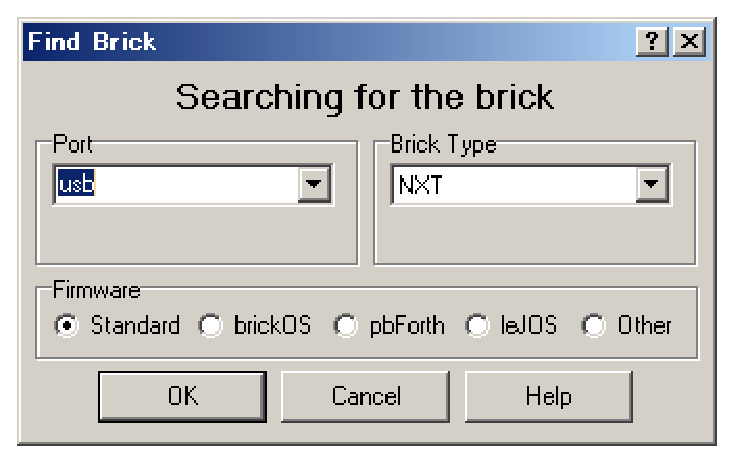
\includegraphics{images/001find_brick.eps}}
  \end{minipage}
\end{center}

 \nmindex{Bricx}を初めて起動すると上のような、LEGO MindStorm接続先を設定する画面が出てきます。
LEGO MindStormをUSBケーブルでパソコンへ接続し、以下のように設定して[OK]を押してください。
\begin{itemize}
\item Port:usb
\item Brick Type:NXT
\item Firmware:Standard
\end{itemize}
接続先を設定せずにBricxを起動したり、LEGO MindStormを接続せずに[OK]を押した場合などには、
\textbf{接続先の再設定}が必要な場合があります。
この場合 Bricxメニューの``Tools''より``Find Brick''を選択すると、
上記の面画が出てきて再設定ができます。

\subsection{プログラムを書いてみよう}

\begin{center}
  \begin{minipage}[t]{10cm}\centering
    \resizebox{10cm}{!}{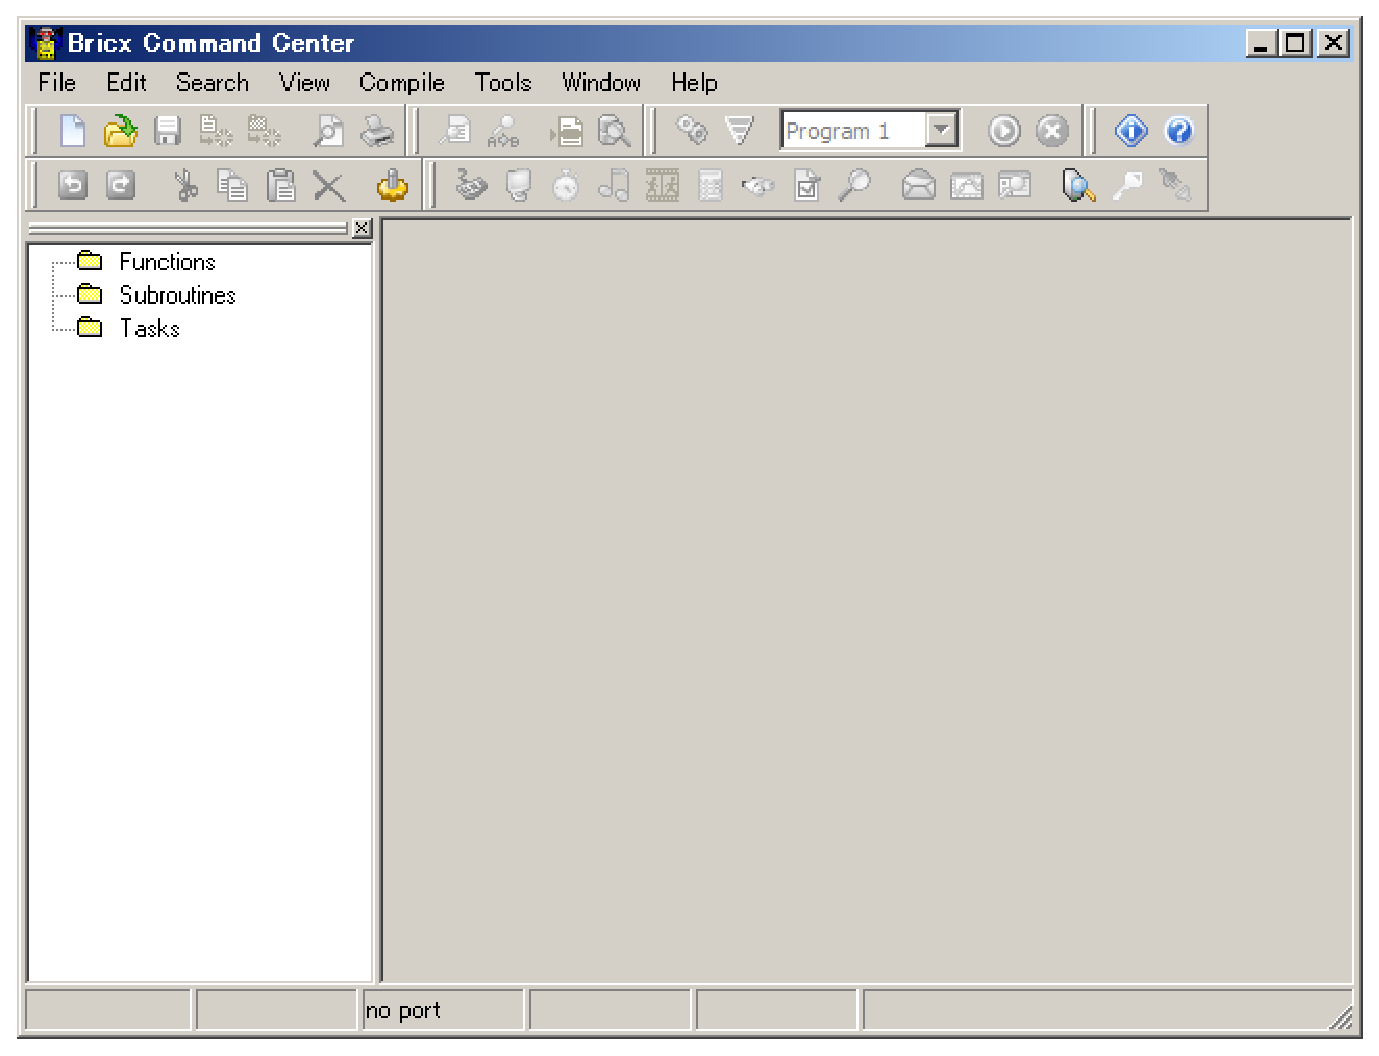
\includegraphics{images/002bricx_command_center.eps}}
  \end{minipage}
\end{center}
% ========================================
% 001find_brick.eps
% 002bricx_command_center.eps
% を入れる
% ========================================


Bricxを起動すると上のような画面がでてきます。
``File''メニューから``New''を選択して以下のようなプログラムを書いてみましょう。

\index{OnFwd()}
\index{OnRev()}<\index{Wait()}
\index{Off()}
\begin{screen}{\small
\begin{verbatim}
task main()
{
  OnFwd(OUT_A, 75); // Aポート(OUT_A)のモータを75%の力で前進方向(Forward)に動かす
  OnFwd(OUT_C, 75); // Cポート(OUT_C)のモータを75%の力で前進方向(Forward)に動かす
  Wait(4000);     // 4秒(4000ms)待つ
  OnRev(OUT_AC, 75); // A,Cポート(OUT_AC)のモータを75%の力で逆向き(Reverse)に動かす
  Wait(4000);     // 4秒待つ
  Off(OUT_AC);    // A,Cポートのモータを止める
}
\end{verbatim}}
\end{screen}
各行において\verb|//|より後の文は\nmindex{コメント}とみなされます。
C言語と同様に\verb|/* */|ではさむこともできます。

% \index{OUT_A}
% \index{OUT_C}
% \index{OUT_AC}
\index{OnFwd}
\index{Wait}
\index{OnRev}
\index{Off}

\subsection{プログラムを実行する}
%\begin{center}
%!!ここにボタン画像を入れる!!
%\end{center}

% ================================
% 003cmpl_dl_run_stop.epsをいれる
% ================================
\begin{center}
  \begin{minipage}[t]{8cm}\centering
    \resizebox{8cm}{!}{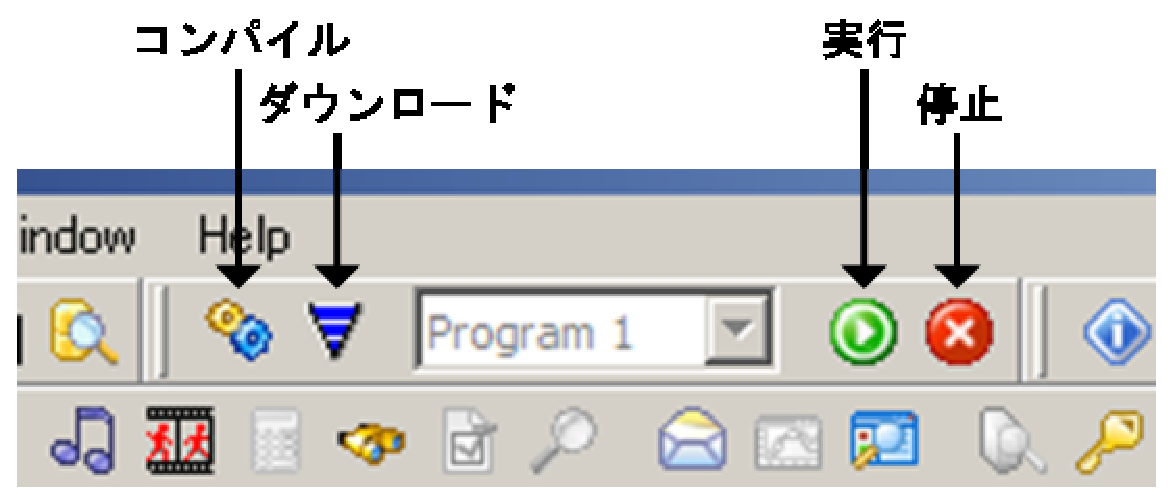
\includegraphics{images/003cmpl_dl_run_stop.eps}}
  \end{minipage}
\end{center}

Bricxの上部のメニューボタンを左から順に押せば,`` \nmindex{compile}"(\nmindex{コンパイル}),
`` \nmindex{download}"(MindStormへ \nmindex{ダウンロード}),``
\nmindex{run}"(\nmindex[じっこう]{実行}),``
\nmindex{stop}"(\nmindex[ていし]{停止})となります。

プログラムをMindStormにインストールした後は,\textbf{USBケーブルをはずして
MindStormのボタンを操作してもプログラムの実行はできます}。

\subsection{プログラムにエラーがおきた時}
コンパイル時にエラー行がハイライト表示されます。

% ================================
% 004error.epsをいれる
% ================================

\begin{center}
  \begin{minipage}[t]{10cm}\centering
    \resizebox{10cm}{!}{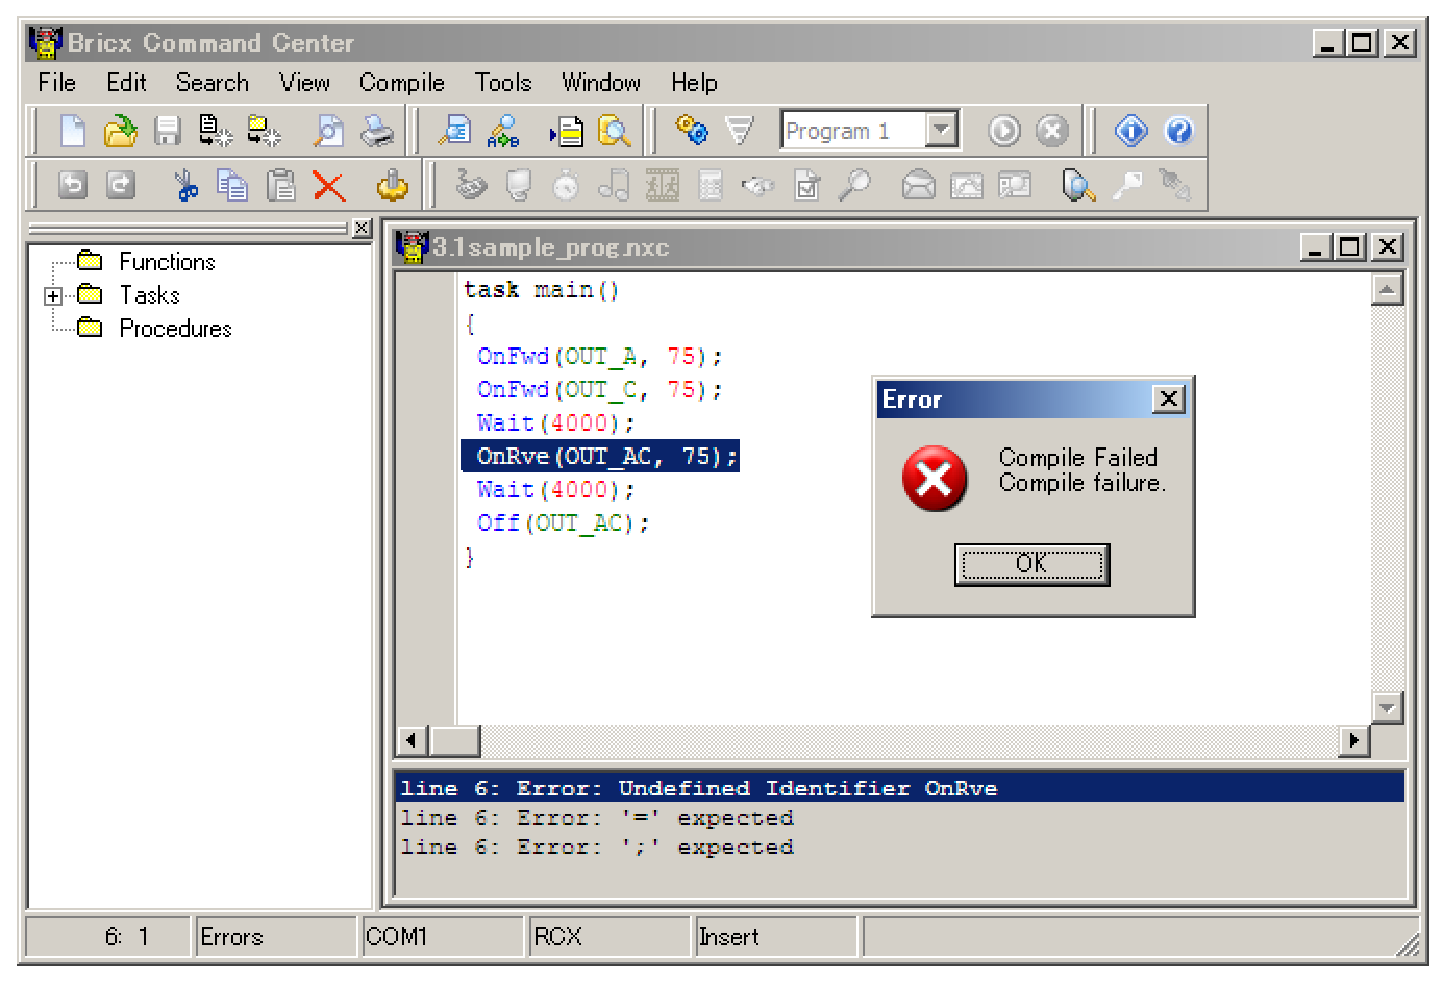
\includegraphics{images/004error.eps}}
  \end{minipage}
\end{center}

\subsection{モータのスピードを変える}
モータのスピードを変えるのは簡単です。以下の例では\nmindex[モータのしゅつりょく]{モータの出力}を$30%$にし,
また前の例よりもプログラムが短くなるように修正してあります。
\begin{screen}{\small
\begin{verbatim}
task main() 
{ 
  OnFwd(OUT_AC, 30); 
  Wait(4000); 
  OnRev(OUT_AC, 30); 
  Wait(4000); 
  Off(OUT_AC); 
}
\end{verbatim}}
\end{screen}

\question
少しバックしてから向きを変えて$3$秒前進するプログラムを作りましょう。


\section{プログラミング入門}

\subsection{変数を使う}

NXCでは,C言語のように\nmindex[へんすう]{変数}を使うこともできます。
NXCには以下のような変数の型があります。

\index{byte}
\index{int}
\index{unsigned int}
\index{short}
\index{long}
\index{unsigned long}
\index{bool}
\index{float}
\index{string}
\index{struct}
\begin{quote}
  \begin{tabular}{lcr}
    \multicolumn{1}{l}{byte} & \dots & \multicolumn{1}{l}{整数型(8bit unsigned,0$\sim$255)} \\
    \multicolumn{1}{l}{int} & \dots & \multicolumn{1}{l}{整数型(16bit,-32,768$\sim$32,767)} \\
    \multicolumn{1}{l}{unsigned int} & \dots & \multicolumn{1}{l}{整数型(16bit unsigned,0$\sim$65,535)} \\
    \multicolumn{1}{l}{short} & \dots    &  \multicolumn{1}{l}{整数型(16bit,intと同じ)} \\
    \multicolumn{1}{l}{long} & \dots    &  \multicolumn{1}{l}{整数型(32bit,-2,147,483,648$\sim$2,147,483,647)} \\
    \multicolumn{1}{l}{unsigned long} & \dots & \multicolumn{1}{l}{整数型(32bit unsigned,0$\sim$4,294,967,295)} \\
    \multicolumn{1}{l}{float} & \dots    &  \multicolumn{1}{l}{浮動小数点型(32bit)} \\
    \multicolumn{1}{l}{bool} &  \dots       &  \multicolumn{1}{l}{trueかfalseの二値をとる変数型} \\
    \multicolumn{1}{l}{string} & \dots      &  \multicolumn{1}{l}{文字変数型}  \\
   \multicolumn{1}{l}{struct} & \dots & \multicolumn{1}{l}{構造体}
\end{tabular}
\end{quote}

NXCには浮動小数的型の変数がないことに気をつけましょう。

\subsubsection{演算子と基本的な関数}

NXCでは以下のような\nmindex[えんざんし]{演算子}や関数を使うことができます。

\begin{center}
\begin{tabular}{lll}  \\ \hline
\multicolumn{1}{c}{オペレータ} & \multicolumn{1}{c}{意味} & \multicolumn{1}{c}{例}  \\ \hline\hline
abs() & 絶対値  & abs()    \\  
sign()  & 符号 & sign()  \\ \hline
$++,--$  & 値を$1$増やす,減らす & $x++$  \\ \hline
$!$              & NOT &  $!x$  \\ \hline 
$*,/$, \% & 掛け算,割り算,余り & $x*y$  \\ \hline
$+,-$    & 足し算,引き算       &   $x+y$   \\ \hline
$<, >$   & 比較                                      &   $x<y$  \\
$==,!=$ &                               &  $x==1$  \\ \hline
$\&\&$       & AND                             & $x\&\&y$  \\ \hline
$\mid\mid$  & OR                             & $x\mid\mid y$  \\ \hline

\end{tabular}
\end{center}


\subsubsection{配列}

\nmindex[はいれつ]{配列}は以下のように宣言します。配列の各要素は$0$に初期化されます。

\index{ArrayInit()}
\begin{screen}{\small
\begin{verbatim}
task main() 
{ 
  int myArray[10][10];  //10×10の配列を宣言 
  int myVector[10];   //大きさ10の配列を宣言
} 
\end{verbatim}}
\end{screen}


\subsubsection{変数の使用例}

\question
下のプログラムを修正して\verb|values[0]|〜\verb|values[3]|の値を
MindStormのLCDディスプレイに表示するようにしなさい。
\begin{screen}{\small
\begin{verbatim}
int aaa; 
int bbb,ccc; 
int values[]; 
task main() 
{ 
  aaa = 5; 
  bbb = 2 * aaa; 
  ccc = bbb; 
  ccc /= 2; 
  aaa *= (ccc + 3);  
  ArrayInit(values, 0, 10);   //配列valuesを大きさ10として各要素値を0にする 
  values[0] = aaa; 
  values[1] = bbb; 
  values[2] = aaa*bbb; 
  values[3] = ccc; 
  NumOut(10, LCD_LINE1, aaa); //LCDディスプレイの1行目(LCD_LINE1),左から10画素の位置に数値表示
  NumOut(10, LCD_LINE2, bbb); //LCDディスプレイの2行目(LCD_LINE2),左から10画素の位置に数値表示
  NumOut(10, LCD_LINE3, ccc); //LCDディスプレイの3行目(LCD_LINE3),左から10画素の位置に数値表示
  Wait(2000);                 //2秒経ったら終わり
} 
\end{verbatim}}
\end{screen}

\subsubsection{乱数}
\index{Random()}
以下は関数\verb|Random()|を使って\nmindex[らんすう]{乱数}を発生したプログラム例です。
関数\verb|Random()|の詳細やその他の数学関数については\ref{sec:math}節を参照し
てください。
\begin{screen}{\small
\begin{verbatim}
int move_time, turn_time; 
task main() 
{ 
  while(true)            // 無限ループ
  {              
    move_time = Random(600);   // 0から600の範囲で乱数発生
    turn_time = Random(400);    //  0から400の範囲で乱数発生 
    OnFwd(OUT_AC, 75); 
    Wait(move_time); 
    OnRev(OUT_A, 75); 
    Wait(turn_time); 
  } 
} 
\end{verbatim}}
\end{screen}


\subsection{制御構文}

\subsubsection{条件式}

\nmindex[ifぶん]{if文}等の\nmindex[じょうけんしき]{条件式}には以下の表現が使えます。

\begin{center}
\begin{tabular}{ll}  \\ \hline
条件式 &  意味  \\ \hline\hline
true    &  常に真  \\ 
false  &  常に偽  \\ 
expr  &  exprの値が$0$でなければ真 \\ \hline
expr1$==$expr2  &  以下いずれもC言語と同様  \\
expr1 $!=$ expr2  &     \\
expr1 $<$ expr2   &   \\
expr1 $<=$ expr2  &  \\
expr1 $>$ expr2     &  \\
expr1 $>=$ expr2  &  \\
$!$ condition            &  \\
cond1 $\&\&$ cond2 &  \\ 
cond1 $\mid\mid$ cond2    &  \\ \hline
\end{tabular}
\end{center}



\subsubsection{if 文,while文}
\nmindex[ifぶん]{if文}や\nmindex[whileぶん]{while文}もC言語と同様に使えます。

\question 以下のプログラムの動作を説明しなさい。

\index{\#define}
\begin{screen}{\small
\begin{verbatim}
#define MOVE_TIME    500  // C言語と同様にマクロ定義も使用可(以下の行にあるMOVE_TIMEは
               // 500に置き換えられる)
#define TURN_TIME    360 
task main() 
{ 
  while(true) 
  { 
    OnFwd(OUT_AC, 75); 
    Wait(MOVE_TIME); 
    if (Random() >= 0)   // Random()はint型(-32,768〜32,767)の乱数を返す 
    { 
      OnRev(OUT_C, 75); 
    } 
    else 
    { 
      OnRev(OUT_A, 75); 
    } 
    Wait(TURN_TIME); 
  } 
} 
\end{verbatim}}
\end{screen} 

\subsubsection{do$\sim$while文}
以下のように \nmindex[dowhileぶん]{do$\sim$while文}も使うことができます。
\begin{screen}{\small
\begin{verbatim}
do 
{ 
  ...
} 
while (condition); 
\end{verbatim}}
\end{screen}

\question
以下のプログラムの動作を説明しなさい。

\begin{screen}{\small
\begin{verbatim}
int move_time, turn_time, total_time; 
task main() 
{ 
  total_time = 0; 
  do 
  { 
    move_time = Random(1000); 
    turn_time = Random(1000); 
    OnFwd(OUT_AC, 75); 
    Wait(move_time); 
    OnRev(OUT_C, 75); 
    Wait(turn_time); 
    total_time += move_time; 
    total_time += turn_time; 
  } 
  while (total_time < 20000); 
  Off(OUT_AC); 
} 
\end{verbatim}}
\end{screen}
do文ではまず\verb|do|に続く\verb|{}|内の命令を一度実行した後に,\verb|while()|で指定した条件がテストされることに
気をつけましょう。




\subsubsection{repeat文}

\index{repeatぶん@repeat文}
\verb|repeat(n){}|を使うと,$n$回同じことをくり返す命令を作れます。
\begin{screen}{\small
\begin{verbatim} 
#define MOVE_TIME    500
#define TURN_TIME    500 
task main() 
{ 
  repeat(4) 
  { 
    OnFwd(OUT_AC, 75); 
    Wait(MOVE_TIME); 
    OnRev(OUT_C, 75); 
    Wait(TURN_TIME); 
  } 
  Off(OUT_AC); 
} 
\end{verbatim}}
\end{screen}

repeat文は,多重ループにすることもできます。

\begin{screen}{\small
\begin{verbatim}
#define MOVE_TIME   1000 
#define TURN_TIME    500 
task main() 
{ 
  repeat(10) 
  { 
    repeat(4) 
    { 
      OnFwd(OUT_AC, 75); 
      Wait(MOVE_TIME); 
      OnRev(OUT_C, 75); 
      Wait(TURN_TIME); 
    } 
  } 
  Off(OUT_AC); 
} 
\end{verbatim}}
\end{screen}


\subsubsection{until 文}

\index{untilぶん@until文}
\begin{screen}{\small
\begin{verbatim}
until (condition)
{
  ...
}
\end{verbatim}}
\end{screen}
until 文は,条件が満たされている限り\verb|{}|内の文がくり返し実行されます。


\subsection{センサー}
MindStormでは様々なセンサーを利用できます。
ロボットの入力ポート$1$に\nmindex{タッチセンサ}を,
% 入力ポート$2$に\nmindex[おとせんさ]{音センサ}を,
入力ポート$2$に\nmindex[ひかりセンサ]{光センサ}を,
入力ポート$3$に\nmindex{カラーセンサ}を,
入力ポート$4$に\nmindex[ちょうおんぱせんさ]{超音波センサ}を接続してく
ださい。
カラーセンサは地面に向けてつけましょう。
\begin{center}
  \begin{minipage}[t]{4cm}\centering
    \resizebox{4cm}{!}{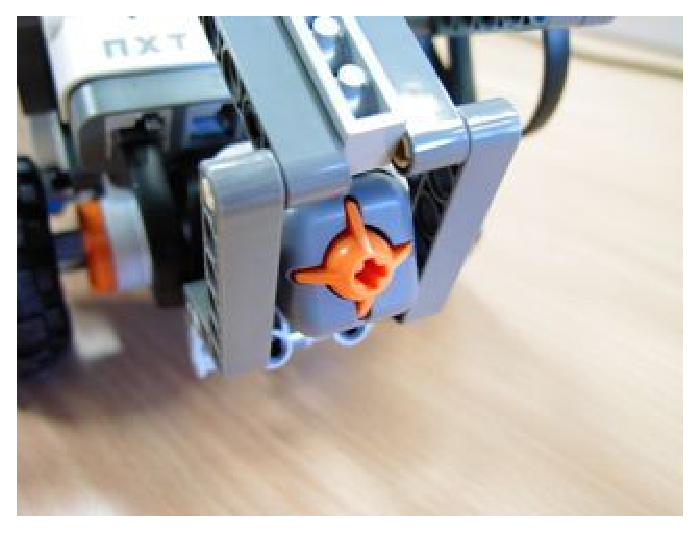
\includegraphics{images/Touch.eps}}\\
    タッチセンサ
  \end{minipage}
  \begin{minipage}[t]{4cm}\centering
    \resizebox{4cm}{!}{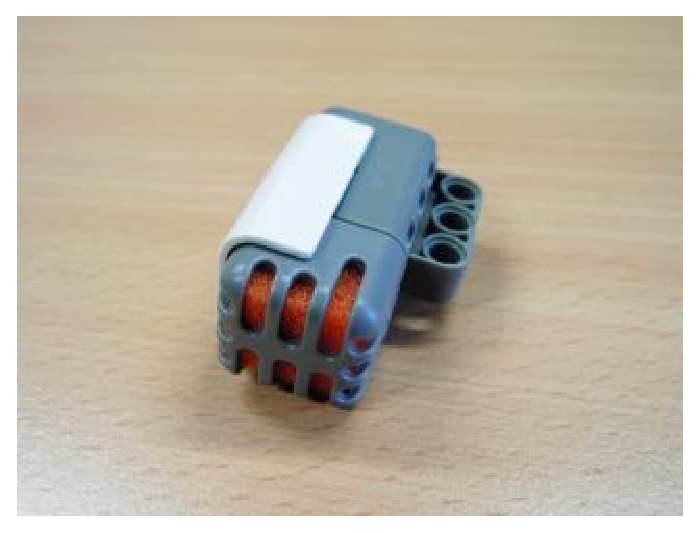
\includegraphics{images/Sound.eps}}\\
    音センサ
  \end{minipage}
  \begin{minipage}[t]{4cm}\centering
    \resizebox{4cm}{!}{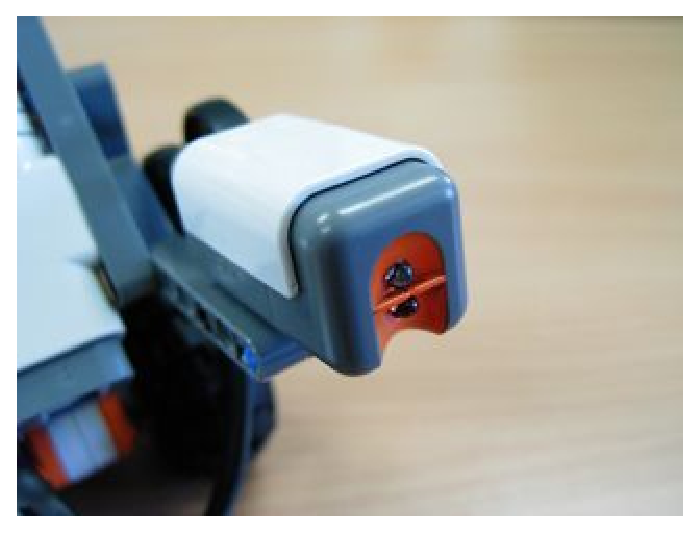
\includegraphics{images/Photo.eps}}\\
    光センサ
  \end{minipage}
  \begin{minipage}[t]{4cm}\centering
    \resizebox{4cm}{!}{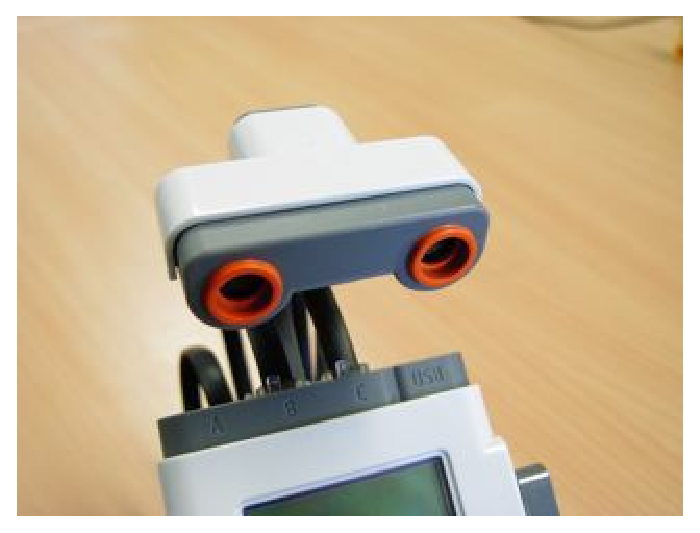
\includegraphics{images/UltraSonic.eps}}\\
    超音波センサ
  \end{minipage}
  \begin{minipage}[t]{4cm}\centering
    \resizebox{4cm}{!}{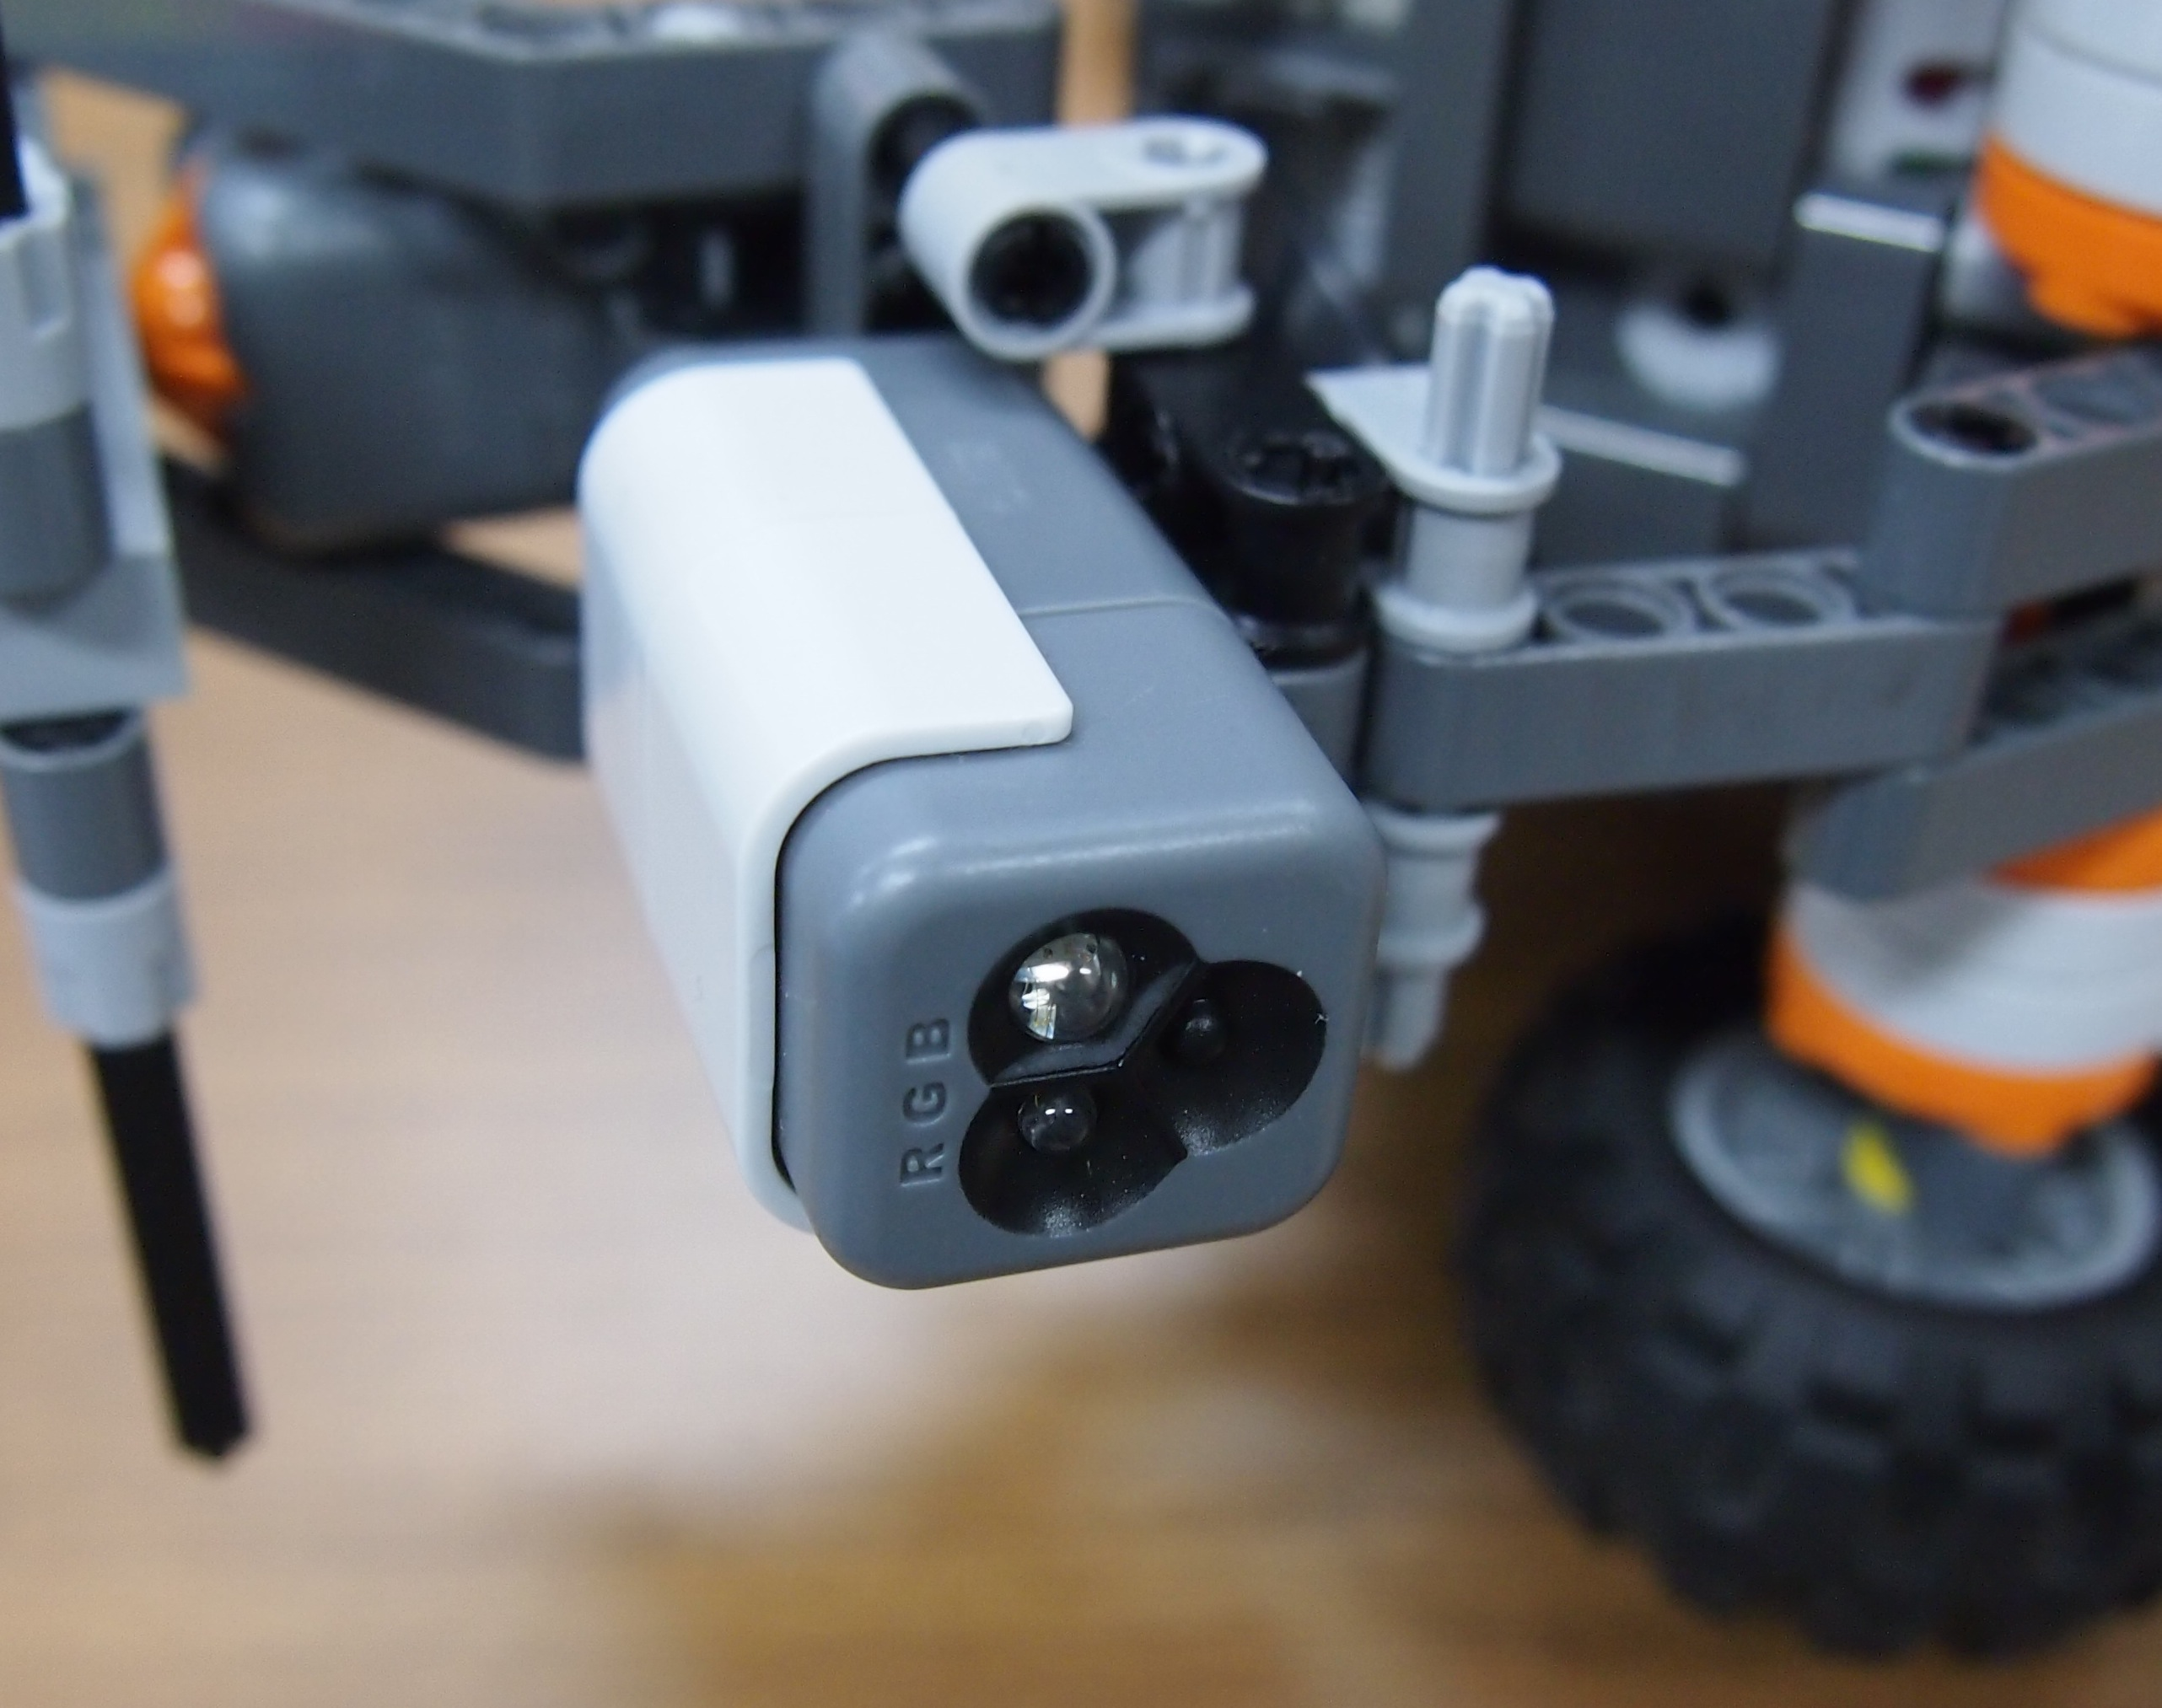
\includegraphics{images/Color.eps}}\\
    カラーセンサ
  \end{minipage}
\end{center}

\subsubsection{センサ入力を待つ}
以下は何かにぶつかるまで直進するプログラム例です。
\begin{screen}{\small
\begin{verbatim}
task main() 
{ 
  SetSensor(IN_1,SENSOR_TOUCH); //入力ポート1にタッチセンサが接続
  OnFwd(OUT_AC, 75); 
  until (SENSOR_1 == 1);        //SENSOR_1は入力ポート1のセンサ値を示す
  Off(OUT_AC); 
} 
\end{verbatim}}
\end{screen}
\index{SetSensor()}
関数\verb|SetSensor()|は MindStormのどの
\nmindex[にゅうりょくぽーと]{入力ポート}にどのようなセンサが接続されているかを指定します。
入力ポートの指定はポート番号に応じて\verb|IN_1|から\verb|IN_4|で行います。

\subsubsection{タッチセンサを使う}
タッチセンサが物体に接触しているかどうかを$1$(接触),$0$(非接触)のセンサ値で知ることができます。

以下は障害物に当たったら少し後ろに下がってから向きを変えて動き続けるプログラム例です。

\begin{screen}{\small
\begin{verbatim}
task main() 
{ 
  SetSensorTouch(IN_1);     //SetSensor (IN_1, SENSOR_TOUCH)と同じ意味
  OnFwd(OUT_AC, 75); 
  while (true) 
  { 
    if (SENSOR_1 == 1)      //センサ値が1(衝突時)かどうかチェック
    { 
      OnRev(OUT_AC, 75); Wait(300); 
      OnFwd(OUT_A, 75); Wait(300); 
      OnFwd(OUT_AC, 75); 
    } 
  } 
}
\end{verbatim}}
\end{screen}
\index{SetSensorTouch()}
関数\verb|SetSensorTocuch()|は接触センサーがどのポートに接続されているか
を指定する命令です。


\subsubsection{光センサを使う}

光センサを使うと,明るさを$0$から$100$までの数値で知ることができます。
以下は明るい時には前進,暗い時には後向きに回転するプログラムです。
光センサの値はMindStormのLCDディスプレイに表示されます。
LCDディスプレイへの表示方法の詳細は\ref{sec:LCD}節を参照してください。
\begin{screen}{\small
\begin{verbatim}
#define THRESHOLD 40 
task main() 
{ 
  int s;
  SetSensorLight(IN_2,false); //入力ポート2に光センサを接続. 
  while (true) 
  { 
    s=Sensor(IN_2);              //Sensor(IN_2)のかわりにSENSOR_2としてもよい
    TextOut(15, LCD_LINE1,"Light:", true); //1行目(LCD_LINE1)の左から15画素の位置に文字列表示
    NumOut(60, LCD_LINE1, s);    //1行目(LCD_LINE1)の左から60画素の位置にセンサ値表示
    if (s>THRESHOLD) { 
      OnFwd(OUT_AC, 75); 
    } else {
      OnRev(OUT_C, 75); 
    }
  } 
} 
\end{verbatim}}
\end{screen}
\index{SetSensorLight()}
関数\verb|SetSensorLight()|は光センサーがどのポートに接続されているか
を指定する命令です。
関数\verb|Sensor()|は指定した入力ポートからの入力値を返り値とする関数
です.

\textbf{光センサーの横のLEDが発光することで反射光の強度を測りたいときには},
\verb|SetSensorLight()|の第二変数で\verb|SetSensorLight(IN_2,true)|
と指定するか,これを省略して\verb|SetSensorLight(IN_2)|とします。
LEDは消灯したままでよければ\verb|SetSensor(IN_2, SENSOR_LIGHT)|を代わ
りに使うことも出来ます。

\question
上記のプログラムを改造して,明るいところでは右に,暗いところでは左に
ロボットが曲がるプログラムを作ってみましょう。
THRESHOLDの値は周囲の明るさよって変更が必要な場合があります。


\subsubsection{カラーセンサを使う}
カラーセンサを使うと,赤, 青, 緑の色情報を数値情報として知る
ことができます。単に明るさ情報を取得して,光センサーの代わりに使うこと
もできます。
以下は地面の明るさや色の情報を
MindStormのLCDディスプレイに表示するプログラムです。
LCDディスプレイへの表示方法の詳細は\ref{sec:LCD}節を参照してください。
\begin{screen}{\small
\begin{verbatim}
task main() 
{ 
  unsigned int r,g,b;
  SetSensorColorFull(IN_3); //入力ポート3に光センサを接続. 
  while (true) 
  { 
    r=ColorSensorValue(IN_3,INPUT_RED);
    g=ColorSensorValue(IN_3,INPUT_GREEN);
    r=ColorSensorValue(IN_3,INPUT_BLUE);
    TextOut(15, LCD_LINE1,":", true); //1行目に明るさ表示
    TextOut(15, LCD_LINE2,"Red:  ", true);   //2行目に赤色の強度
    TextOut(15, LCD_LINE3,"Green:", true); //3行目に緑色の強度
    TextOut(15, LCD_LINE4,"Blue: ", true);  //4行目に青色の強度
    NumOut(60, LCD_LINE1, (r+g+b)/3);
    NumOut(60, LCD_LINE2, r);
    NumOut(60, LCD_LINE3, g);
    NumOut(60, LCD_LINE4, b);
    Wait(500);
  } 
} 
\end{verbatim}}
\end{screen}
\index{SetSensorColorFull()}
関数\verb|SetSensorLight()|はカラーセンサーがどのポートに接続されているか
を指定する命令です。
この命令では\textbf{カラーセンサーの横のLEDが発光することで色情報を取
  得できますが},LEDを消灯したい時にはかわりに
\verb|SetSensorColorNone(IN_2)|を使います。



\question
上記のプログラムを改造して,カラーセンサを使って地面に書いた黒い線にそって
ロボットを動かすプログラムを作ってみましょう。
黒い線の右端に沿って動くプログラムと,左端に沿って動くプログラムの両方
を作ってみてください。
THRESHOLDの値やモータ出力は周囲の明るさやコースによって変更が必要な場
合があるのでいろいろなコースで試してみましょう。

\subsubsection{音センサを使う}
以下はポート2に音センサを接続したプログラム例です。

\begin{screen}{\small
\begin{verbatim}
#define THRESHOLD 40 
#define MIC SENSOR_2 
task main() 
{ 
  SetSensorSound(IN_2);    //入力2に音センサ接続. SetSensor(IN_2, SENSOR_SOUND)と同じ意味
  while(true){ 
     until(MIC > THRESHOLD); //while (MIC<THRESHOLD); でもよい
     OnFwd(OUT_AC, 75); 
     Wait(300);          //なくても良いが,あると動きが(多分)ややスムーズになる
     until(MIC > THRESHOLD); 
     Off(OUT_AC); 
     Wait(300); 
  } 
} 
\end{verbatim}}
\end{screen}
\index{SetSensorSound()}
関数\verb|SetSensorSound()|は音センサーを接続したポート番号を指定する
命令です。

\question 上記のプログラムの動作を説明しなさい。
また実際にプログラムをロボットに実行させ,
2つのWaitの有無による動作の違いを考察しなさい。


\subsubsection{超音波センサを使う}
超音波センサは,出した音が返ってくるまでの時間を計ることで前方の物体までの距離を測ることができるセンサです。

\question 以下のプログラムの動作を説明し,実際にロボットを使って動作確認をしなさい。

\begin{screen}{\small
\begin{verbatim}
#define NEAR 15 //cm 
task main(){ 
  SetSensorLowspeed(IN_4); //入力4に超音波センサ接続. SetSensor(IN_4, SENSOR_LOWSPEED)でも良い
  while(true){ 
    OnFwd(OUT_AC,50); 
    while(SensorUS(IN_4)>NEAR); 
    Off(OUT_AC); 
    OnRev(OUT_C,100); 
    Wait(800); 
  } 
} 
\end{verbatim}}
\end{screen}
\index{SetSensorLowspeed()}
関数\verb|SetSensorLowspeed()|は超音波センサがどのポートに接続されているか
を指定する命令です。
\index{SensorUS()}
ここで,\textbf{超音波センサによって対象物まで距離を知るには関数}\verb|SensorUS()|\textbf{を使う}事に気をつ
けましょう。\verb|SensorUS()|は超音波センサのセンサ値から距離(cm)に変換して返す関数です.

\question
超音波センサのセンサ値をLCDディスプレイに表示するプログラムを作って、
超音波センサで測れる距離の範囲を確認しなさい。
超音波センサは小さなものには反応しにくいので、大きめの紙や板を使って
試すこと。

\subsection{TaskとFunctions}

\subsubsection{Tasks}
NXCには\bfindex[へいれつけいさん]{並列計算}の機能があり,複数の作業を同時に行う事ができます。
\textbf{並列して実行できる作業単位}を\bfindex{task}と呼びます.
task は1つのプログラム中に最大255個まで作ることができます。
taskの定義方法は後の例で示すようにC言語の関数と似ています.
プログラム中にtask mainは必ず1つだけ作る必要があります。
プログラム実行時にはtask mainがまず呼び出されます。
他のtaskはtask mainから関数Precedes()使って呼び出します。
この場合,task mainの実行終了後にPrecedes()で呼び出した関数の実行が始
まります。

以下はロボットが障害物に当たったら,方向転換しながら動き回るプログラム例です。
ロボットは直進するというtaskである\verb|move_forward()|と,タッチセンサ
の入力を監視しながら入力があれば方向転換をするというtaskである
\verb|check_sensors()|を並列して行っています。

\begin{screen}{\small
\begin{verbatim}
mutex mFlag; 
task move_forward() 
{ 
  while (true) 
  { 
    Acquire(mFlag);        //他のタスクが手旗を取ってなければここで取る(mFlagをAcguire)
    OnFwd(OUT_AC, 75);
    Release(mFlag);         //手旗を放す(mutexを解放(Release))
  } 
} 
task check_sensors() 
{ 
  while (true) 
  { 
    if (SENSOR_1 == 1) 
    { 
      Acquire(mFlag);       //他のタスクが手旗を取ってなければここで取る
      OnRev(OUT_AC, 75); Wait(500); 
      OnFwd(OUT_A, 75); Wait(500); 
      Release(mFlag);        //手旗を放す
    } 
  } 
} 
task main() 
{ 
  Precedes(move_forward, check_sensors);//2つのタスクを並列処理することを指定
  SetSensorTouch(IN_1);              //task mainの終了後,指定したtaskの実行がはじまる
} 
\end{verbatim}}
\end{screen}

タスクmainで呼び出している関数\nmindex{Precedes}は並列計算をする複数のtaskを呼び出します.
必要に応じて3つ以上のtaskを引数として指定して呼び出す事もできます。

2つのtaskを同時に実行していると,その2つのタスクが1つのモータに異なる方向に動くように命令を出してしまう
可能性があります。
このような問題を防ぐため,\bfindex{mutex} (mutual exclusion,相互排除)という型の変数を使います。
上の例ではmutex型の変数mFlagを2つのtaskが関数\nmindex{Acquire()}でとりあいをしています。
一方がmFlagのAcquire(獲得)に成功していれば,
\index{Release()}Release(解放)されるまで,もう一方のtaskはAcquireできず,その後の命令は実行されません。
このようなmutex型の変数は\bfindex{semaphore}(手旗信号)と呼ばれ,並列計算で一般によく使われます。


\subsubsection{関数(Functions)}
C言語の関数とほぼ同じものとしてNXCにも関数(Function\index{function})が
あります。
関数はtaskから呼び出す事もできますし,関数から他の関数を呼び出す事もで
きます。

ロボットに(1)何事もなければ直進,(2)ぶつかったら方向転換,という動作を
させたい時には(1),(2)に対応するtaskを書いて並列処理をします。この2つ
のtaskの実現に必要な実行単位(前進する,後進するなど)は関数で作って
taskから呼び出すことができます。
並列処理が不要ならtask main以外のtaskは作らなくてもよいです。

\begin{screen}{\small
\begin{verbatim}
void turn_around(int pwr)  // 関数の宣言はC言語と同様
                  // この例ではvoidとしてもよい
{ 
  OnRev(OUT_C, pwr); Wait(900); 
  OnFwd(OUT_AC, pwr); 
} 
task main() 
{ 
  OnFwd(OUT_AC, 75); 
  Wait(1000); 
  turn_around(75);        //先に定義した関数を呼び出す
  Wait(2000); 
  turn_around(75); 
  Wait(1000); 
  turn_around(75); 
  Off(OUT_AC); 
} 
\end{verbatim}}
\end{screen}

この例では関数の返り値voidですが,C言語と同様にintやstringを返り値にすることもできます。

\subsubsection{引数のアドレス渡し}
以下は関数への引数の\bfindex[あどれすわたし]{アドレス渡し}の例です。
C言語のようにポイントを使うかわりに,NXCでは引数に\&をつけることでアド
レス渡しを実現できます。
(C++言語と同じ書式です。)

\begin{screen}{\small
\begin{verbatim}
void foo(int &x)   //引数のアドレス渡し 
{ 
  x = 2; 
} 
task main() 
{ 
  int y = 1;        // yに1を代入
  foo(y);          // yは2になります
  foo(2);         // アドレス渡しの場合は引数は変数でないとダメ
} 
\end{verbatim}}
\end{screen}

\subsubsection{並列タスク}

\question 以下のプログラムの悪い点を指摘し,修正案を書きなさい。
\begin{screen}{\small
\begin{verbatim}
task check_sensors() 
{ 
  while (true) 
  { 
    if (SENSOR_1 == 1) 
    { 
      OnRev(OUT_AC, 75); 
      Wait(500); 
      OnFwd(OUT_A, 75); 
      Wait(850); 
    } 
  } 
} 
task forward() 
{ 
  while (true) 
  { 
    OnFwd(OUT_AC, 75); Wait(100); 
  } 
} 
task main() 
{ 
  SetSensor(IN_1,SENSOR_TOUCH); 
  Precedes(check_sensors, forward); 
} 
\end{verbatim}}
\end{screen}

\question
ライントレースをしながら,ライン上にあった障害物にぶつかりそうになったら,
もしくはぶつかったら少し後ろに下がってからランダムに方向転換してラインを探し、
ラインを見つけたらまたライントレースをするプログラムを並列タスクを利用し
て作りましょう。


\subsection{LCDディスプレイ表示\label{sec:LCD}}
MindStormには100x64画素のLCDディスプレイがあります。
以下はLCDディスプレイに文字や数値を出力するプログラム例です.
原点座標(0,0)はディスプレイの左下の位置です.

\begin{screen}{\small
\begin{verbatim}
#define X_MAX 99
#define Y_MAX 63
#define X_MID (X_MAX+1)/2
#define Y_MID (Y_MAX+1)/2
task main(){
  int i = 1234;
  TextOut(15, LCD_LINE1,"Display", true);//左から15画素,LCD_LINE1(1行目)の位置に文字列表示
  NumOut(60,LCD_LINE1, i);              //左から60画素,LCD_LINE1(1行目)の位置に数値表示
  PointOut(1,Y_MAX-1);
  PointOut(X_MAX-1,Y_MAX-1);
  PointOut(1,1);
  PointOut(X_MAX-1,1);
  Wait(200);
  RectOut(5,5,90,50);
  Wait(200);
  LineOut(5,5,95,55);
  Wait(200);
  LineOut(5,55,95,5);
  Wait(200);
  CircleOut(X_MID,Y_MID-2,20);
  Wait(800);
  ClearScreen();
  GraphicOut(30,10,"faceclosed.ric"); Wait(500);
  ClearScreen();
  GraphicOut(30,10,"faceopen.ric");
Wait(1000);
}
\end{verbatim}
}
\end{screen}

上記のプログラムで使っている関数の詳細は以下の通りです.
\index{ClearScreen()}
\index{NumOut()}
\index{TextOut()}
\index{GraphicOut()}
\index{CircleOut()}
\index{LineOut()}
\index{PointOut()}
\index{RectOut()}
\index{ResetScreen()}
\begin{center}
\begin{tabular}[t]{l|l}\hline
関数名 & 機能 \\\hline
\verb|ClearScreen()| & 画面を消す\\
\verb|NumOut(x, y, number)| & (x,y)の位置に数値numberを表示\\
\verb|TextOut(x, y, string, clear=false)| & (x,y)の位置に文字stringを表示。第4引数をtrueとすると\\
& 画面消去後表示\\
\verb|GraphicOut(x, y, filename)| & .ric形式の画像データを表示(ric形式)\\
\verb|CircleOut(x, y, radius)| & 中心(x,y), 半径radiumの円を描く\\
\verb|LineOut(x1, y1, x2, y2)| & (x1,x2) と (x2,y2) を直線で結ぶ\\
\verb|PointOut(x, y)| & (x,y)に点を描く\\
\verb|RectOut(x, y, width, height)| & 四角形を描く。(x,y):左下の座標, width:幅, height:高さ\\
\verb|ResetScreen()| & 画面をリセットする\\\hline
\end{tabular}
\end{center}

\question
MindStormの各センサ(超音波センサ,光センサ)の値の一覧を画面に表示するプ
ログラムを作りましょう。

\subsection{ファイル入出力}


NXCでファイルにアクセスするにはbyte型の変数をファイルアクセス用に用意します。
これがC言語のファイルポインターのような役目をします。

以下はファイルにデータを書き出すプログラム例です。
このプログラムではまず,これから作りたいファイル(``\verb|Danny.txt|'')がすでにあればこれを
消してからファイルを作成しています。
\index{CreateFile()}次にCreateFile関数でファイルを開きます。
この時ファイルの大きさをバイトで指定する必要があることに注意して下さい。
ファイルはLEGOの本体のメモリ内に作られます。
このため\textbf{あまり大きなファイルは作れない}ことによく注意しましょ
う。
また\textbf{不要になったファイルは必ず直ちにMindStorm内から消してください}.

\index{WriteLnString()}
\verb|WriteLnString (fileHandle, string, bytesWritten)|は
\nmindex{fileHandle}の指すファイルに文字列stringを書き出します。その後
何バイト書き出されたかが変数bytesWrittenに代入されます。

\index{DeleteFile()}
\index{CreateFile()}
\index{CloseFile()}
\index{StrCat()}
\index{WriteLnString()}
\begin{screen}{\small
\begin{verbatim}
task main(){ 
   byte fileHandle;       // ファイルアクセスのための変数を用意 
   short fileSize; 
   short bytesWritten; 
   string read;        // 文字列readを宣言 
   string write;        // 文字列Writeを宣言
   DeleteFile("Danny.txt");  // Danny.txtを消す
   CreateFile("Danny.txt", 512, fileHandle);  // 512バイトの大きさのファイルを開く
   for(int i=2; i<=10; i++ ){ 
      write = "NXT is cool "; 
      string tmp = NumToStr(i);            // 数値を文字列に変換してtmpに代入
      write = StrCat(write,tmp," times!");    // 引数で与えた3つの文字列をStrictで
                             // つなげて変数writeに代入
      WriteLnString(fileHandle,write, bytesWritten);   // 文字列writeを書き出す
   } 
   CloseFile(fileHandle);                    // ファイルを閉じる
} 
\end{verbatim}}
\end{screen}


結果を見るには,BricxCC$\rightarrow$Tools$\rightarrow$NXT Explorerをクリックして,
\verb|upload Danny.txt|でファイルをPCにアップロードしてみて下さい。

以下は数値データをファイルに書き出し,その後ファイルのデータを読み込んでMindStormのLCDディスプレイに
表示するプログラム例です。

\index{OpenFileRead()}
\index{ClearScreen()}
\index{ReadLn()}
\index{NumOut()}
\begin{screen}{\small
\begin{verbatim}

task main () { 
   byte handle, time = 0; 
   int n, fsize,len, i; 
   int in; 
   DeleteFile("int.txt"); 
   CreateFile("int.txt",4096,handle);     // 4096バイトまで書けるファイルを作る 
   for (int i = 1000; i<=10000; i+=1000){ 
      WriteLn(handle,i);              // ; の値を書き出し
   } 
   CloseFile(handle);               // ファイルを閉じる
   OpenFileRead("int.txt",fsize,handle);    // ファイルを読み出しモードで開く
   until (ReadLn(handle,in)!=NO_ERR){      // 1行読んで結果をinに代入
      ClearScreen();        // 画面消去
      NumOut(30,LCD_LINE5,in);  // 5行目の行頭から30画素の位置にinの値を書く
      Wait(500); 
   } 
   CloseFile(handle);       // ファイルを閉じる
} 
\end{verbatim}}
\end{screen}



\section{発展的なプログラミング}

\subsection{LEDライトを点灯する}
接続したLEDライトの点灯や消灯はモータの制御と同様に行ないます。
たとえばBポートにライトをつけている場合は以下のようにします。
\begin{screen}
\begin{verbatim}
OnFwd(OUT_B,70); //点灯
Off(OUT_B);  //消灯
\end{verbatim}
\end{screen}

\subsection{音楽を鳴らす}
NXTはいろいろな高さの音や音源ファイルを鳴らすこともできます。
音を鳴らすには関数\index{PlayToneEx()}
PlayToneEx(frequency, duration, volume, loop?)を使います。
frequencyは周波数(Hz),durationは長さ(ms),volumeは強さ(0から4),
そしてloop?には一度だけ鳴らすならFALSEもしくは0を,くり返すならTRUEもしくは1を指定します。

\index{PlayTone()}PlayTone(frequency, duration)を使うこともできます。
この場合の音の強さは一定(NXTのメニューで設定)になります。
以下は周波数の一覧表です。

\begin{center}{\small
\begin{tabular}{ll|ccccccc}  \\ \hline
    \multicolumn{2}{c|}{\textbf{Sound}} &    \textbf{3}&       \textbf{4}&       \textbf{5}&          \textbf{6}&        \textbf{7}&            \textbf{8}&    \textbf{9}  \\  \hline
シ&B &        247&  494&   988&  1976&  3951&  7902&      \\
ラ\verb|#|&A\verb|#|  &       233&  466&  932 &  1865&  3729&  7458&       \\
ラ&A&       220&   440&  880&  1760&  3520&  7040&  14080\\ 
ソ\verb|#|&G\verb|#|&           &  415  &  831  &  1661  &  3322  &  6644  &  13288 \\
ソ&G   &          &  392  &  784  &  1568  &  3136  &  6272  &  12544 \\ 
ファ\verb|#|&F\verb|#| &           &  370  &  740  &  1480  &   2960  &  5920  &  11840 \\ 
ファ&F   &           &  349  &  698  &  1397  &  2794  &  5588  &  11176 \\
ミ&E   &           &  330  &  659  &  1319  &  2637  &  5274  &  10548 \\ 
レ\verb|#|&D\verb|#| &          &   311  &  622  &  1245  &  2489  &  4978  &  9956 \\ 
レ&D   &          &  294  &  587  &  1175  &  2349  &  4699  &  9398  \\ 
ド\verb|#|&C\verb|#| &         &   277  &  554  &  1109  &  2217  &  4435  &  8870 \\  
ド&C   &         &  262  &  523  &  1047  &  2093  &  4186  &  8372 \\ \hline
\end{tabular}}
\end{center}


\index{PlayFileEx()}PlayFileExを使うと1つの音が終わる前に次のコマンドが実行されるので,\verb|Wait|コマンドで音と音の間隔を調節する必要があります。

\begin{screen}{\small
\begin{verbatim}
#define VOL 3 
task main() 
{ 
  PlayToneEx(262,400,VOL,FALSE);  Wait(500); 
  PlayToneEx(294,400,VOL,FALSE);  Wait(500); 
  PlayToneEx(330,400,VOL,FALSE);  Wait(500); 
  PlayToneEx(294,400,VOL,FALSE);  Wait(500); 
  PlayToneEx(262,1600,VOL,FALSE); Wait(2000); 
} 
\end{verbatim}}
\end{screen}

BricxCCを使っている方は\nmindex{BrickPiano}で簡単に曲を作ることもできます。MindStormで曲を鳴らしたい時は曲をTaskにして
プログラムを組むことをおすすめします。以下は例です。

\begin{screen}{\small
\begin{verbatim}
task music() 
{ 
  while (true) 
  { 
    PlayTone(262,400);  Wait(500); 
    PlayTone(294,400);  Wait(500); 
    PlayTone(330,400);  Wait(500); 
    PlayTone(294,400);  Wait(500); 
  } 
} 
task movement() 
{ 
  while(true) 
  { 
    OnFwd(OUT_AC, 75); Wait(3000); 
    OnRev(OUT_AC, 75); Wait(3000); 
  } 
} 
task main() 
{ 
  Precedes(music, movement); 
} 
\end{verbatim}}
\end{screen}


\subsection{関数のマクロ定義}
C言語のように,\index{\#define}\verb|#define|を使って定数だけでなく関数のマクロ定義をすることもできます。

\begin{screen}{\small
\begin{verbatim}
#define turn_around  \ 
  OnRev(OUT_B, 75); Wait(3400);OnFwd(OUT_AB, 75);  // 以下のTurn_aroundという文字列は,                  // コンパイル前にOnRev・・・,という文字列におきかえられる
task main() 
{ 
  OnFwd(OUT_AB, 75); 
  Wait(1000); 
  turn_around; 
  Wait(2000); 
  turn_around; 
  Wait(1000); 
  turn_around; 
  Off(OUT_AB); 
} 
\end{verbatim}}
\end{screen}

\verb|#define|の定義は1行で書く必要があります。
\textbf{1行で入らない時は行末に}\verb|"\"|\textbf{を書いて改行していることを明示}して下さい。

以下は引数も使ったマクロ関数の定義の例です。

\begin{screen}{\small
\begin{verbatim}
#define turn_right(s,t)  \ 
  OnFwd(OUT_A, s);OnRev(OUT_B, s);Wait(t); 
#define turn_left(s,t)   \ 
  OnRev(OUT_A, s);OnFwd(OUT_B, s);Wait(t); 
#define forwards(s,t)    OnFwd(OUT_AB, s);Wait(t); 
#define backwards(s,t)   OnRev(OUT_AB, s);Wait(t); 
task main() 
{ 
  backwards(50,10000); 
  forwards(50,10000); 
  turn_left(75,750); 
  forwards(75,1000); 
  backwards(75,2000); 
  forwards(75,1000); 
  turn_right(75,750); 
  forwards(30,2000); 
  Off(OUT_AB); 
} 
\end{verbatim}}
\end{screen}



\subsection{inline関数}

短い関数を作るときには以下のように\nmindex{inline}宣言をして下さい。
この場合,関数を呼び出した場所に関数の実行内容が展開されます。
その結果メモリは多く必要になりますが,処理速度は速くなります。

\begin{screen}{\small
\begin{verbatim}
inline int Name( Args ) { 
   return x*y; 
}
\end{verbatim}}
\end{screen}

以下は例です。


\begin{screen}{\small
\begin{verbatim}
inline void turn_around() 
{ 
  OnRev(OUT_C, 75); Wait(900); 
  OnFwd(OUT_AC, 75); 
} 
task main() 
{ 
  OnFwd(OUT_AC, 75); 
  Wait(1000); 
  turn_around(); 
  Wait(2000); 
  turn_around(); 
  Wait(1000); 
  turn_around(); 
  Off(OUT_AC); 
} 
\end{verbatim}}
\end{screen}

上記のinline関数に引数を作った例が以下です。

\begin{screen}{\small
\begin{verbatim}
inline void turn_around(int pwr, int turntime) 
{ 
  OnRev(OUT_C, pwr); 
  Wait(turntime); 
  OnFwd(OUT_AC, pwr); 
} 
task main() 
{ 
  OnFwd(OUT_AC, 75); 
  Wait(1000); 
  turn_around(75, 2000); 
  Wait(2000); 
  turn_around(75, 500); 
  Wait(1000); 
  turn_around(75, 3000); 
  Off(OUT_AC); 
} 
\end{verbatim}}
\end{screen}



\appendix
\section{用意されている数学関数\label{sec:math}}

\index{Random()}
{\large \textbf{
Random(n)}
}
\begin{verbatim}
  0からn-1までの値の乱数(整数)を返す
   x=Random(10);      // 0から9までの値を返す
\end{verbatim}


{\large \textbf{
Random()}
}
\begin{verbatim}
  int型(-32,768〜32,767)の乱数を返す
   x=Random();
\end{verbatim}

\index{Sqrt()}
{\large \textbf{
Sqrt(x)}
}
\begin{verbatim}
  xの平方根(整数)を返す
   x=Sqrt(x);
\end{verbatim}


\index{Sin()}
{\large \textbf{
Sin(degrees)}
}
\begin{verbatim}
  指定した角度に対するSin関数の値を100倍した整数値 (-100から100)を返す
   x=Sin(theta);
\end{verbatim}

\index{Cos()}
{\large \textbf{
Cos(degrees)}
}
\begin{verbatim}
  指定した角度に対するCos関数の値を100倍した整数値 (-100から100)を返す
   x=Cos(y);
\end{verbatim}

\section{トラブル対策}
\begin{itemize}
\item MindStormを接続したUSBが認識されない。
  \begin{itemize}
  \item MindStormのドライバを管理者権限でインストールしましょう。
    一般ユーザ権限でインストールしているとMindStormとは接続できないの
    で気をつけてください。
  \end{itemize}
\item プログラムをコンパイルできない。
  \begin{itemize}
  \item bricx(zipファイル)をダウンロードしたまま解凍しないでbricxを起
    動していませんか?
  \item bricxの実行形式のみを(アイコンをドラッグして持っていって)
    デスクトップ等にコピーして使ってませんか。
    コピーの代わりにショートカットを使うか,Bricxのフォルダの中の実行
    形式を直接実行しましょう
  \item プログラムのエラーメッセージが出てないか確認しましょう。
  \end{itemize}
\item プログラムをMindStormにダウンロードが出来ない。
  \begin{itemize}
  \item \ref{sec:bricx}節を参照してPort, Brick Type, Firmwareの設定を確認
    してください。
  \item MindStormに古いプログラムが多数残っていると, ダウンロードのた
    めのメモリが足りなくなることがあります。この場合はMindStormを操作
    して不要なプログラムを消してください。
  \item MindStormのドライバを一般ユーザ権限でインストールしていると
    MindStormと接続できません。管理者権限でインストールしてください。
  \end{itemize}
\end{itemize}

\printindex
\end{document}
